\section{Solving Identification with a Control Function (CF)}
\label{sec:selectionmodel}
If your goal is to estimate CM effects, and you could control for unobserved selection terms $U_{0,i}, U_{1,i}$, then you would.
This ideal (but infeasible) example would yield unbiased estimates for the ADE and AIE.
% Alas, $U_i$ is by definition unobserved.
A Control Function (CF) approach takes this insight seriously, providing conditions to model the implied confounding by $U_{0,i}, U_{1,i}$, and then controlling for it.

The main problem is that second-stage reqression equation \eqref{eqn:parametric-secondstage} is not identified, because $U_{0,i},U_{1,i}$ are unobserved.
\begin{align}
    \label{eqn:secondstage-reg}
    \Egiven{Y_i}{Z_i, D_i, \vec X_i} \;\; =& \;\;
        \alpha
        + \beta D_i
        + \gamma Z_i
        + \delta Z_i D_i
        + \varphi(\vec X_i) \\
        & \;\; +\left( 1 - D_i \right) \Egiven{ U_{0,i} }{D_i = 0, \vec X_i}
            + D_i \Egiven{ U_{1,i} }{D_i = 1, \vec X_i} 
        \nonumber
\end{align}

CF methods were first devised to correct for sample selection problems \citep{heckman1974shadow}, and were extended to a general selection problem \citep{heckman1979sample}.
The approach works in the following manner: (1) assume that the variable of interest follows a selection model, where unexplained first-stage selection informs unobserved second-stage confounding; (2) extract information about unobserved confounding from the first-stage; and (3) incorporate this information as control terms in the second-stage equation to adjust for selection-into-mediator.
Identification in CF methods typically relies on either distributional assumptions about the unobserved error terms in the second-stage, or exclusion restrictions provided by instrumental variables in the first-stage, or both.
By explicitly accounting for the information contained in the first-stage selection model, CF methods enable consistent estimation of causal effects in the second-stage even when selection is driven by unobserved factors \citep{florens2008identification}.

In the example of analysing health gains from health insurance \citep{finkelstein2008oregon}, a CF approach could be used to address the unobserved confounding from not observing underlying health conditions.
It would do so by assuming that unobserved selection-into-more frequent health care usage is informative for underlying health conditions; this assumes people with more sever underlying conditions visit the doctor (weakly) more often than those without.
Then it includes this information in the estimation of how much the effect goes through increased usage of healthcare (i.e., the ADE and AIE).

\subsection{Re--identifying Causal Mediation (CM) Effects}
The following assumptions are sufficient to model the correlated error terms, identifying $\beta, \gamma, \delta$ in the second-stage regression \eqref{eqn:secondstage-reg}, and thus both the ADE and AIE.
\theoremstyle{definition}
\newtheorem{assumptionCF}{Assumption}
\renewcommand\theassumptionCF{CF--\arabic{assumptionCF}}
\begin{assumptionCF}
    \label{cf:monotonicity}
    Mediator monotonicity.
    \[ \Probgiven{ D_i(1) \geq D_i(0) }{\vec X_i} = 1. \]
\end{assumptionCF}

Assumption \ref{cf:monotonicity} is the monotonicity condition first used in an instrumental variables context \citep{imbens1994identification}.
Explain in here the selection model implication, $D = 1{ \phi(Z, X) > V }$ which can be transformed into $D = 1{ \pi(Z, X) > U }$ for $U_i = F_V(V_i) ~ unif(0, 1)$.

\begin{assumptionCF}
    \label{cf:identification}
    Selection on costs and benefits.
    \[ \Cov{U_i, \, U_{0,i}}, \; \Cov{U_i, \, U_{1,i}} \neq 0. \]
\end{assumptionCF}

Explain how the connected errors give you want.
Assuming that first-stage unobserved heterogeneity explains second-stage selection-into-$D_i$.

Suppose the vector of control variables $\vec X_i$ has at least two entries;
denote $\vec X_i^{\text{IV}}$ as one entry in the vector, and $\vec X_i^-$ as the remaining.
\begin{assumptionCF}
    \label{cf:instrument}
    Mediator take-up cost instrument.
    \[ \vec X_i^{\text{IV}} \textnormal{ satisfies }
    \partialdiff{\vec X_i^{\text{IV}}}\left[
        \mu_1(z', \vec X_i) - \mu_0(z', \vec X_i)\right] = 0
        < \partialdiff{\vec X_i^{\text{IV}}}\Egiven{D_i(z')}{\vec X_i},
        \textnormal{ for } z' = 0, 1. \]
\end{assumptionCF}

Explain how the instrument is necessary to separately identify the CF in the first-stage.
Instrument separately identifies the propensity score (not technically required but needed for efficiency).
Assuming that an instrument exists, which satisfies an exclusion restriction (i.e., not impacting mediator gains $\mu_1-\mu_0$), and has a non-zero influence on the mediator (i.e., strong first-stage).
The exclusion restriction is untestable, and must be guided by domain-specific knowledge; strength of the first-stage is testable, and must be justified with data by methods common in the instrumental variables literature.

\newtheorem{proposition}{Proposition}
\begin{proposition}
    \label{proposition:secondstage}
    If assumptions \ref{cf:monotonicity}, \ref{cf:identification}, \ref{cf:instrument} hold, then second-stage regression equation \eqref{eqn:parametric-secondstage} is identified with a CF adjustment.
    \begin{align*}
        \Egiven{Y_i}{Z_i, D_i, \vec X_i} \;\; =& \;\;
            \alpha
            + \beta D_i
            + \gamma Z_i
            + \delta Z_i D_i
            + \varphi(\vec X_i) \\
            & \;\; +  \rho_0 \left( 1 - D_i \right) \lambda_0 \big( \pi(Z_i ; \vec X_i) \big)
                + \rho_1 D_i \lambda_1 \big( \pi(Z_i ; \vec X_i) \big)
    \end{align*}
\end{proposition}

Where $\lambda_0, \lambda_1$ are the CFs.
For $J(u) = F^-1_V(u) - E[ F^-1_V(U_i) ]$

Explain this a selection model thing, either choosing a distribution (and thus $\vec\lambda$), or relying on semi-parametric methods to partial it out.

This is a special case of Heckman (1980), notation from Kline Walters (2019).

\newtheorem{theoremCF}{Theorem}
\renewcommand\thetheoremCF{CF}
\begin{theoremCF}
    \label{thm:cf-identification}
    The ADE and AIE are identified, with parameters identified in the second-stage regression that includes a CF adjustment (Proposition \ref{proposition:secondstage}).
    \begin{align*}
    \text{ADE}
    %= \E{Y_i(1, D_i(Z_i)) - Y_i(0, D_i(Z_i))}
        &= \E{\gamma + \delta D_i}, \\
    \text{AIE}
    %= \E{Y_i(Z_i, D_i(1)) - Y_i(Z_i, D_i(0))}
        &= \E{ \bar \pi
            \Big( \beta +  \delta Z_i +
                (\rho_1 - \rho_0) \,
                \Gamma \big(\pi(0; \vec X_i), \pi(1; \vec X_i) \big)\Big)}.
    \end{align*}
\end{theoremCF}
For $\Gamma\left(p,p'\right) = \frac{p'\lambda_1\left(p'\right) - p\lambda_1\left(p\right)}{p' - p}$, and $\bar\pi = \pi(1; \vec X_i) - \pi(0; \vec X_i)$ the mediator complier score.

\citep{kline2019heckits}.

This is exploiting ideas from selection models + marginal TEs to identify this system, including using the selection model to identify the mediator compilers’ effect.
Indeed, mediation estimates already do a two-step procedure; it is a minor adjustment to include a CF  in the second-stage, to guard against selection-on-gains (chief among which is the Roy model).

\begin{figure}[h!]
    \caption{Simulated Distribution of CM Effect Estimates, Relative to True Value.}
    \begin{subfigure}[c]{0.475\textwidth}
        \centering
        \caption{$\hat{\text{ADE}} - \text{ADE}$.}
        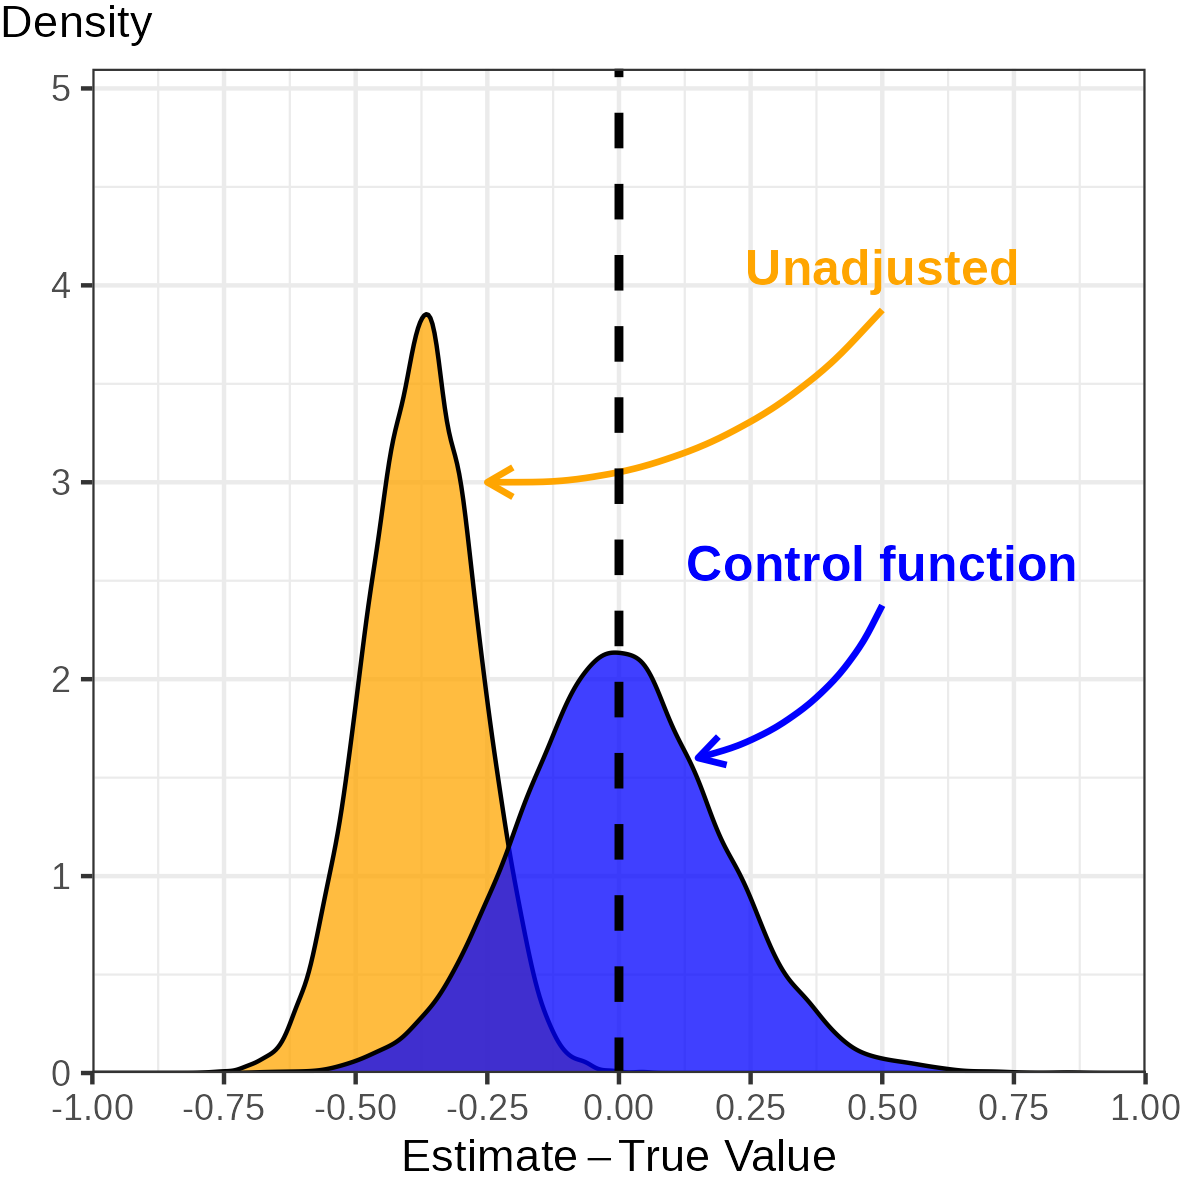
\includegraphics[width=\textwidth]{
            ../programs/simulations/sim-output/heckit-direct-dist.png}
    \end{subfigure}
    \begin{subfigure}[c]{0.475\textwidth}
        \centering
        \caption{$\hat{\text{AIE}} - \text{AIE}$.}
        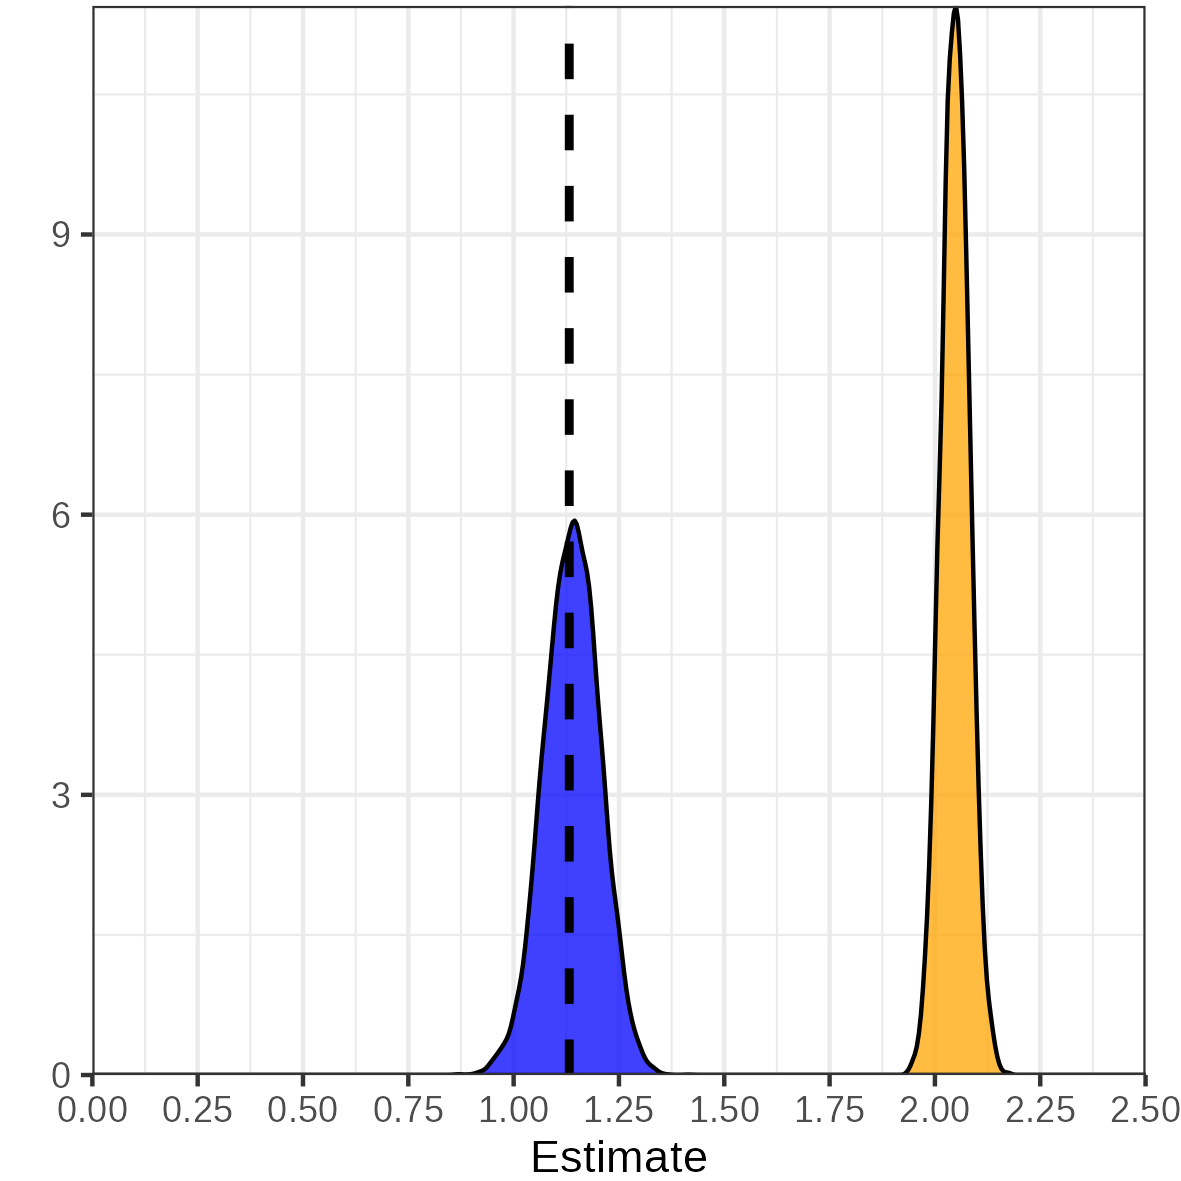
\includegraphics[width=\textwidth]{
            ../programs/simulations/sim-output/heckit-indirect-dist.png}
    \end{subfigure}
    \label{fig:cm-heckit-dist}
    \justify
    \footnotesize    
    \textbf{Note:}
    These figures show the empirical density of point estimates, for 10,000 different datasets generated from a Roy model with correlated normally distributed error terms (further described in \autoref{sec:controlfun}).
    The black dashed line is the true value;
    orange is the distribution of conventional CM estimates from two-stage OLS \citep{imai2010identification},
    and blue estimates with a two-stage Heckman selection adjustment.
\end{figure}
